\chapter{Introduction}
\label{chap:introduction}
% Story on data cleaning, to introduce the subject
This first chapter will cover an introduction to the main research topic and motivation of this thesis in \autoref{sec:errordetection_intro} and \autoref{sec:motivation}. Then the research questions will be introduced in \autoref{sec:researchquestions}. The main contributions will be covered in \autoref{sec:contributions} and lastly, the outline of this thesis will be shown in \autoref{sec:outline}.

\section{Error detection}
\label{sec:errordetection_intro}
% What are errors?
\subsection{A data story}
\label{subsec:data_story}
In 2020, everybody knows the word \textit{data}. Everybody wants to use data to improve their business, their academic work or even their daily lives. However, what does it actually mean to \textit{use data}? To give a clear idea of what \textit{using data} could look like, we take a look at an example scenario of a fictional character named "Robert". 

~\\Robert is working at a local bakery, selling different french baked goods. His bakery sells croissants, baguettes and macarons. Robert heard from a friend that he should use \textit{data} in order to improve his business. He came up with the idea to keep an Excel sheet with all the products that were sold. Then, after a full day of hard work, he wanted to show the owner of the bakery which product contributes the most to the revenue, so that they might focus more on that product. 
At the end of the day, the sheet with looked like this, shown in figure \ref{fig:dirty_data_robert}. Each line (row) of data contains which order number the product belonged to, the product name and price, time sold and the seller of the product.

\begin{figure}
    \centering
    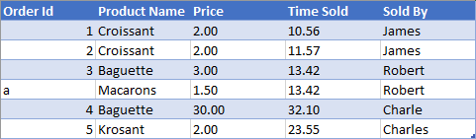
\includegraphics[width=0.9\linewidth]{thesis/Figures/DirtyDataset.png}
    \caption{Roberts data after a day of work}
    \label{fig:dirty_data_robert}
\end{figure}

Because it was the first time gathering data, some of the values might have been entered incorrectly in the Excel sheet. Nevertheless, Robert goes and makes a nice pie chart to show his boss the findings of that day. The graph in figure \ref{fig:sales_pie_dirty} shows the pie chart with revenue contribution for that day.
Immediately, his boss tells him that he does not believe this graph and walks out of the office. 
If you look closely at figure \ref{fig:sales_pie_dirty}, you see that something weird has happened. Suddenly, 4 product categories are shown. "Krosant" does not even exist, so this graph cannot be correct either. Also, it could not be true that the shop got 81\% of their revenue through "Baguette", that did not feel right for Robert. Robert just experienced an example of: \textbf{Garbage in, Garbage out.} Somehow, using the data that was gathered, was not helpful at all.

\begin{figure}[h]
    \centering
    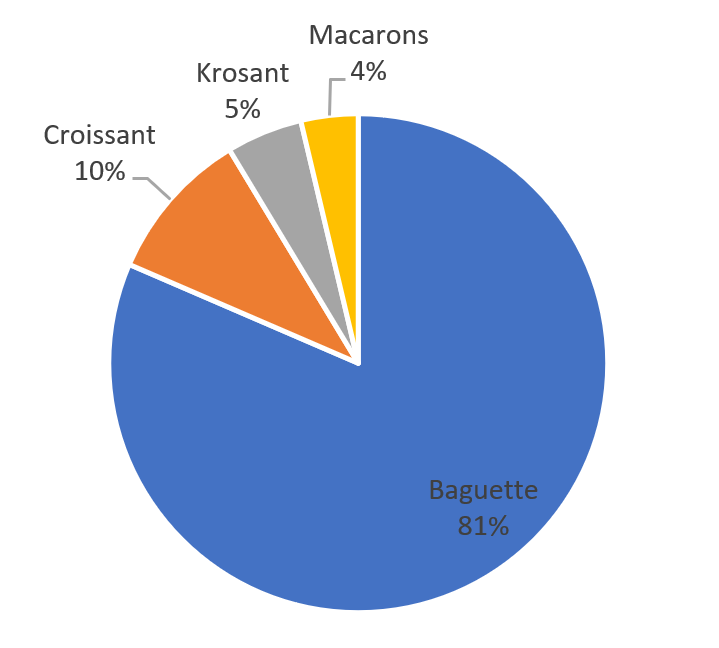
\includegraphics[width=0.5\linewidth]{thesis/Figures/Sales_Pie_Dirty.png}
    \caption{Roberts first revenue contribution chart}
    \label{fig:sales_pie_dirty}
\end{figure}

Robert quickly goes back to his sheet to see what went wrong. Taking a closer look, Robert sees that mistakes have been made. He sees that values in figure \ref{fig:dirty_data_robert} cannot be true, as they do not belong to the values that can be possible. For example, "Krosant" must be "Croissant" and a "Baguette" only sells for 3.00 euros, not 30.00. The values that he altered, were \textbf{errors}. After Robert correct the data, it looked like figure \ref{fig:clean_data_robert}.

\begin{figure}[h]
    \centering
    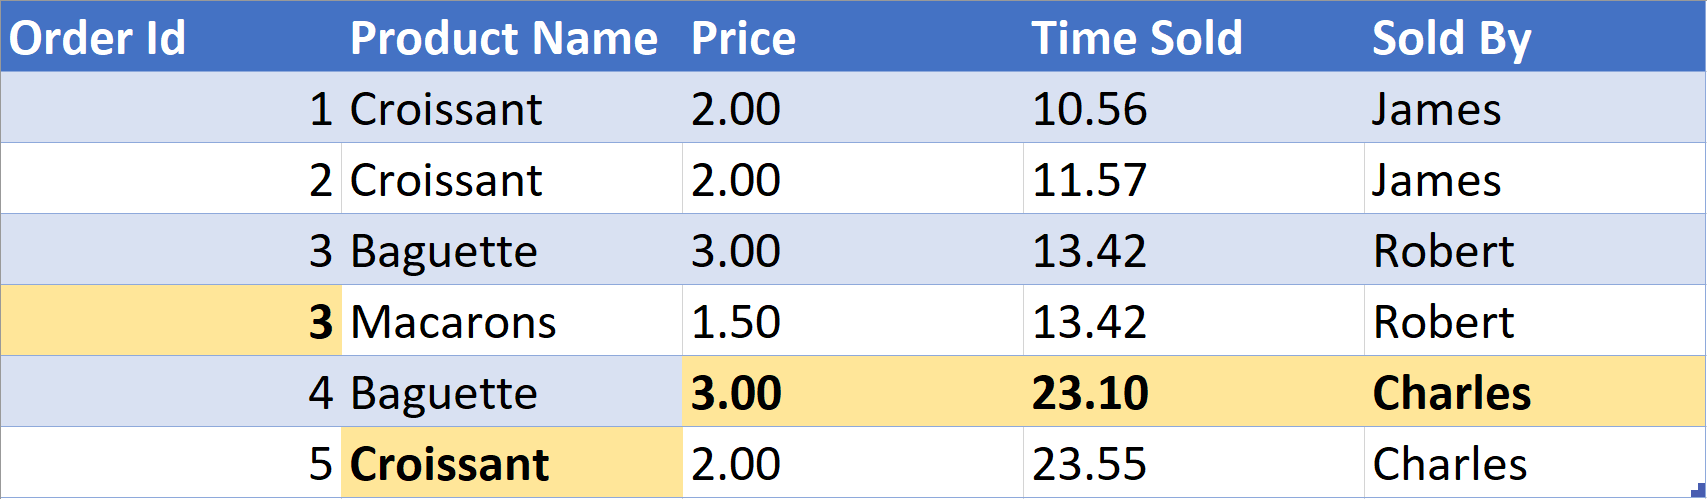
\includegraphics[width=0.9\linewidth]{thesis/Figures/CleanDataset.png}
    \caption{Roberts corrected data}
    \label{fig:clean_data_robert}
\end{figure}

Being more confident that the saved data is better now, Robert creates a new pie chart, as shown in figure \ref{fig:sales_pie_clean}. Going back to his boss, he shows the new results. 
~\\The boss now trusts Roberts results and graph. The chart gives a proper idea on which of the 3 products drive revenue, giving more insights and possibility of acting upon that insight.
And this is all the result of a single chart and well cleaned data!

\begin{figure}[H]
    \centering
    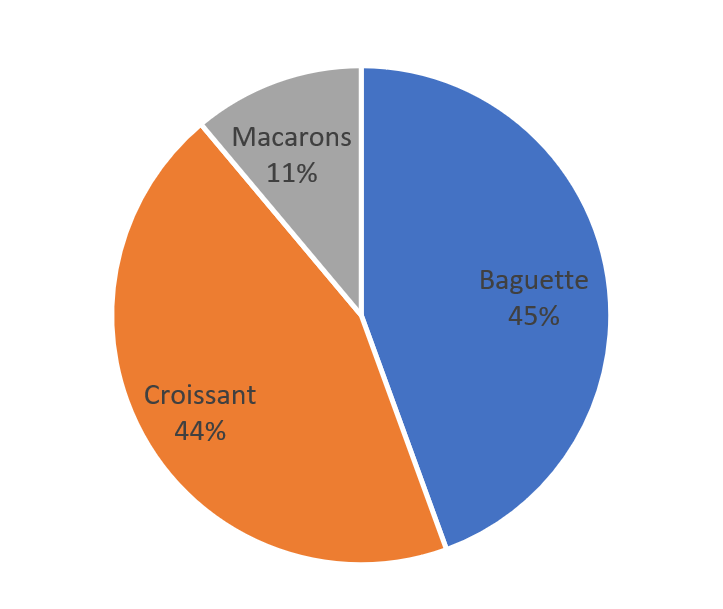
\includegraphics[width=0.5\linewidth]{thesis/Figures/Sales_Pie_Clean.png}
    \caption{Roberts corrected revenue contribution chart}
    \label{fig:sales_pie_clean}
\end{figure}

\subsection{Research topic}
The story told in the previous subsection was a story about using data. It started with collecting data. Then finding out that the collected data was not fit for generating insights. The data had to be cleaned. Data cleaning is a process that is the foundation of every individual or group that wants to do data science.

%% General part
\blockquote{Data cleaning is the process of \textbf{\textit{detecting}} and correcting (or removing) corrupt or inaccurate records from a \textbf{record set, table, or database} and refers to \textbf{identifying incomplete, incorrect, inaccurate or irrelevant parts} of the data and then replacing, modifying, or deleting the dirty or coarse data.}

In this thesis, the research topic will be the data cleaning process. As this process is a fairly broad concept, a more concentrated part will be focused on. Only the first step of data cleaning, the \textit{detection} of dirty data or so-called \textbf{error detection} will be the scope of this research.
As seen in the definition of data cleaning, the goal of error detection is to identify incomplete, incorrect, inaccurate or irrelevant parts of the data. 

% What are errors in relational data sources + what are relational data sources?
Moreover, the focus will be on relational data sources. These types of sources follow the relational model \cite{Codd1970-vj}. This is a structure that presents the data in tuples, or rows. Each row is grouped into relations that are defined for the complete table. A relational dataset has different attributes or columns. Also, each row in that dataset will have a value for these attributes, also called a data cell. Data sources in the relational model are queryable using SQL (Structured Query Language). 

~\\The example data of section \ref{subsec:data_story} is also relational data, as shown in figures \ref{fig:dirty_data_robert} and \ref{fig:clean_data_robert}. While the data in both figures \ref{fig:dirty_data_robert} and \ref{fig:clean_data_robert} refer to the same real-world entities, events or other characteristics, there is a difference between the two. The difference between the two versions is correction of unwanted values to the desired values. The unwanted differences are called errors.
~\\So an error in relational data is a deviation from the desired ground truth values.

% What is the problem? 
~\\The problem a user tries to solve in this domain is to identify all erroneous cells in a relational dataset. In the examples given above, manual cleaning is still possible, but with increasing size of datasets, increasing cost in cleaning arise. Luckily, there exist (semi-)automated error detection tools. These algorithms or tools try to identify erroneous cells, based on common deviations from the ground truth. These common errors could be outlying numerical values (like the "baguette" costing 30.00 euros), missing values or misspellings ("Krosant" vs "Croissant"). Questions that arise when trying to find a tool that helps detecting errors are:

\begin{itemize}
    \item Which algorithm is the best?
    \item How will it perform when I run it on my data?
    \item How to configure that tool?
    \item Why would it work and can we understand when it does not work?
\end{itemize}

These questions are the foundation of the work presented in this thesis. Now that the topic has been introduced, the motivation of the subject will be covered in the next section.
\section{Motivation}
\label{sec:motivation}
% Why is it interesting and important?
Errors in relational data are present in all fields, both in academics as well as in the industry. 

%% Industry & academics
In business, it is known throughout various studies and news articles that the cost of bad data is high. Poor data across businesses and the government cost the U.S. economy \$3.1 trillion a year in 2012 (\cite{Ilyas2015-oh}). Every company nowadays wants to be more 'data-driven', but does not foresee the challenge that arises with processing data. Also, the amount of data created and stored is growing exponentially. The total estimated amount of data stored has grown by an approximated ten-fold since 2012 and will only continue to grow according to industry experts (\autoref{fig:annual_data_size}), to an estimated 175 zettabytes\footnote{1 zettabyte = 1 billion terabytes = $10^{21}$ bytes} by 2025. This growth in data creation will lead to a growth in the amount of poor data and consequently growth in costs if not properly dealt with. 

\begin{figure}
    \centering
    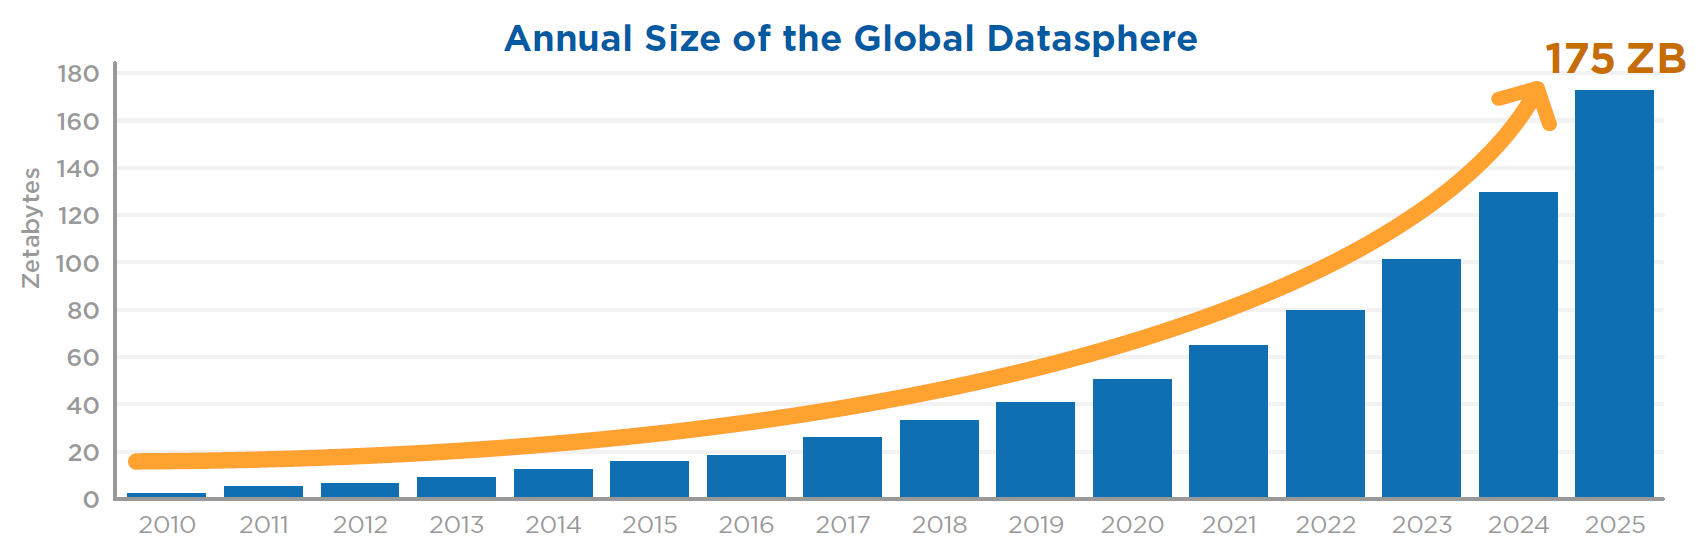
\includegraphics[width=\textwidth]{thesis/Figures/AnnualDataSize.png}
    \caption{Annual size of the global datasphere (\cite{Rydning2018-mt})}
    \label{fig:annual_data_size}
\end{figure}

% Maintain good customer relationships
% Improve organisation efficiency
% Drive useful data-driven insights
% Privacy
Companies want to use data for various reasons, such as: maintaining good customer relationships, improving organisation efficiency and drive useful data-driven insights. And at the same time following all the latest privacy regulations.  
% Pyramid of data cleaning
But, in order to pursue these aspirations and be able to extract value from data, numerous steps have to be taken beforehand. A pyramid of data science or artificial intelligence (AI) needs is shown in \autoref{fig:pyramid_data}. This shows that before any aggregating or learning from data can be done, the data needs to be explored and transformed properly. This is where error detection comes into play. If the data cleaning step with error detection as the foundation is not correctly executed, the upper levels of the data science hierarchy cannot be reached properly. Without data cleaning, valuable actions like analytics, experimentation or even artificial intelligence will not be possible.

\begin{figure}
    \centering
    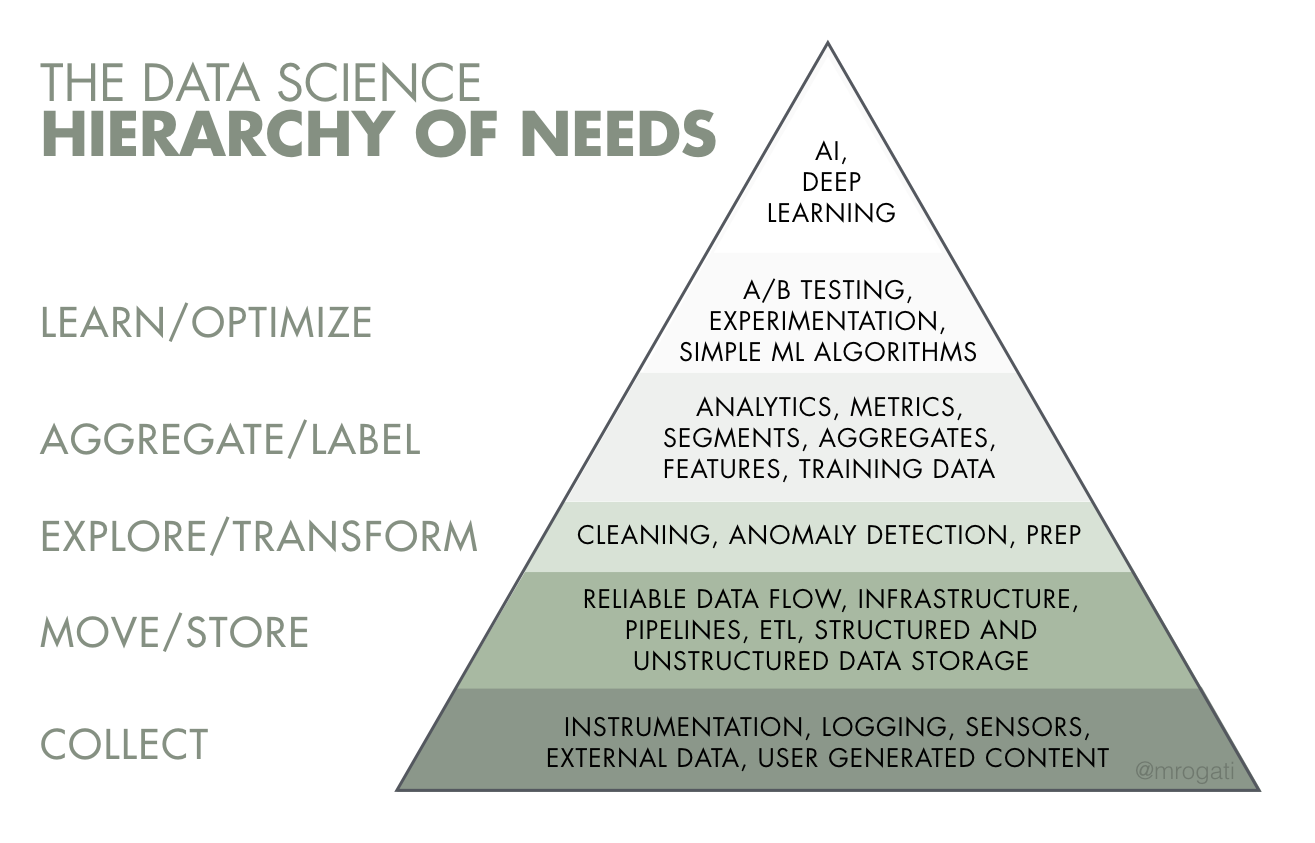
\includegraphics[width=\linewidth]{thesis/Figures/PyramidData.png}
    \caption[The data science hierarchy of needs]{The data science hierarchy of needs\footnotemark}
    \label{fig:pyramid_data}
\end{figure}
\footnotetext{Monica Rogati -  \url{https://hackernoon.com/the-ai-hierarchy-of-needs-18f111fcc007}}

% Academics focus
~\\For the past few years, governments, industry and academics have been investing both money and effort into big data and the data processing pipelines in general (\cite{Cai2015-hr}). As data quality issues in relational data sources have been a pressing problem for the industry for a longer period of time, researchers now try to take learning from experience in the field in corporate businesses (\cite{Stonebraker2018-ag}). Working with industry allows scientists to have access to more resources and real-life examples of the complications of errors in relational data, which could accelerate the solution-finding process. This is beneficial for academics, as the importance of data quality in research is also prevalent. Poor data quality might not have the monetary consequences in academics like it has in business, but bad quality in academics could lead to falsely substantiated conclusions. 

% Why is it hard? (E.g., why do naive approaches fail?)
%% Time consuming
%% Costly to run all
~\\Unfortunately, data cleaning does not have a single solution that is omnipotent and time-efficient. The complexity and heterogeneous nature of relational data make the error detection task more difficult to tackle. There is no single dominant tool for general-purpose error detection and domain-specific tools achieved better precision and recall scores than general-purpose tools (\cite{Abedjan2016-jc}). 
This leads to the difficulty of selecting the right tool for the job, with the right configuration. A user that is not familiar with the range of available options will not be able to select the best tool. Running all tools will be too time-consuming and will not have a guaranteed result. Preferably, a user wants automatic error detection, without the requirement of human expertise or any sort of configuration.

~\\If it even would be possible to provide an automatic tool, without the need of a human expert, new questions arise. 
If a machine learning (ML) model performs well, why do we not just trust the model and ignore why it made a certain decision? "The problem is that a single metric, such as classification accuracy, is an incomplete description of most real-world tasks." (\cite{Molnar2020-do}).
That is where interpretability comes into play. Not all ML systems require interpretability, but those where the problem is not studied and validated enough, or the consequences of unacceptable results are too significant need an explanation of how it works (\cite{Doshi-Velez2017-ec}). Interpret means to explain or to present in understandable terms. Because of the complexity and all different forms relational data can have, error detection in that landscape is too complex and can have too significant consequences to take its workings for granted. 

~\\Whilst there have been many solutions proposed for the task of error detection, there are still many improvements to be made. The following main problems have occurred in recent public work:

\paragraph{Usability problems:} There are many error detection tools and other data cleaning solutions that are not available to the public. Tools that are openly available have their challenges to prepare for usage in real life. Expertise is needed to configure and set up the tools. Also, the input and output formats deviate per tool. 

\paragraph{Completeness problems:} Due to the great amount of error detection tools available and the inherent costs that come with them to run, not all proposed tools in research have been tested on a broad range of datasets. Vice versa, not all types of datasets have been cleaned with the different tools available. This means that there are many unknowns when it comes to the performance of tools in all sorts of datasets or selecting the best tool for a specific dataset.

\paragraph{Interpretability problem:} All proposed tools have underlying common principles and techniques that they are designed to work with. In real-life datasets, these techniques might produce different results than expected. At the moment, no research has used interpretability methods to understand how the error detection tools work in retrospect, after evaluation. This would give better insight if and how the tools would work on unseen real-life datasets, and if there are any hidden side-effects or influences on the performance of these tools.

\section{Research Questions}
\label{sec:researchquestions}
Resulting from this motivation, the following research questions will tried to be answered in this thesis:

\paragraph{\textit{Main Research Question:}} 
~\\\textbf{How to choose a fitting error detection algorithm for a specific relational dataset?}

~\\With the following sub-questions:
\paragraph{RQ1} What is the current state of the art and what is the performance of these tools?

\paragraph{RQ2} Is it possible to create an extensive data profile to estimate performance on unseen datasets?

\paragraph{RQ3} Is it possible to generate a ranking of tools according to their performance on unseen datasets?

\paragraph{RQ4} Do these data profiles provide more interpretability of error detection tools?

\section{Contributions}
\label{sec:contributions}
By answering the research questions above, the following contributions have been made in this research:

\begin{itemize}
    \item An error detection framework with 6 different error detection tools
    \item A comparison study of error detection algorithms for relational data
    \item A suggestion system for error detection tools and configuration for unseen relational datasets
    % \item Method of interpretability 
\end{itemize}

\section{Outline}
\label{sec:outline}
The outline of this thesis is as follows. 
First, in chapter \ref{chap:background}, the background on error detection in relational data is given. Besides the foundational information on error types, scores and error detection benchmarking, state of the art tools and methods will be covered. Also, the background on dataset profiling and interpretability with respect to error detection will be given. 
In chapter \ref{chap:methodology}, the methodology of this research is highlighted, in order to answer the research questions given in \ref{sec:researchquestions}. Specific used datasets, erorr detection tools and machine learning techniques will be covered.
Then, in chapter \ref{chap:results}, the results of the research will be presented. 
In chapter \ref{chap:discussion} the discussion on the research is provided and lastly in chapter \ref{chap:conclusion}, conclusions and future work will be discussed.